\chapter{Database}
\begin{figure}[!htp]
	\centering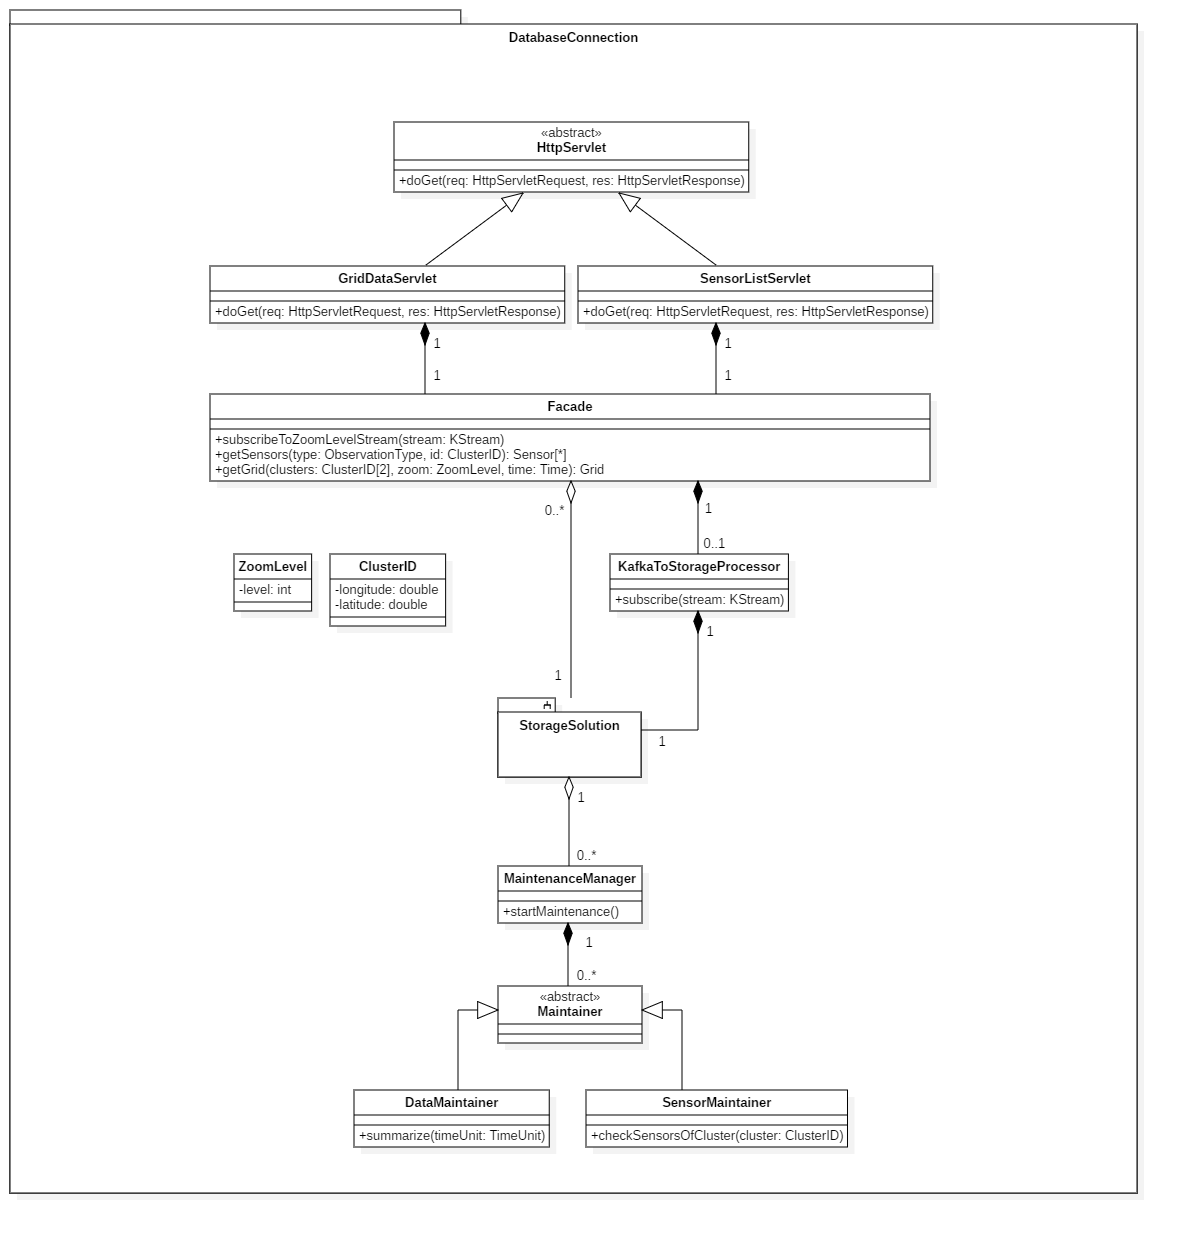
\includegraphics[width=\linewidth]{images/database/DatabaseClassDiagram}
	\caption{Klassendiagramm Database}
\end{figure}
\section{Package DatabaseConnection}{
\label{DatabaseConnection}\hypertarget{DatabaseConnection}{}
\hskip -.05in
\hbox to \hsize{\textit{ Package Contents\hfil Page}}
\vskip .13in
\hbox{{\bf  Classes}}
\entityintro{ClusterID}{DatabaseConnection.ClusterID}{This class describes a unique identification of a cluster via longitude and latitude.}
\entityintro{DataMaintainer}{DatabaseConnection.DataMaintainer}{This class maintains the sensordata in the StorageSolution.}
\entityintro{Facade}{DatabaseConnection.Facade}{A facade to simplify access to a StorageSolution, such as a database.}
\entityintro{GridDataServlet}{DatabaseConnection.GridDataServlet}{An HTTPServlet for requesting Grid data.}
\entityintro{HttpServlet}{DatabaseConnection.HttpServlet}{An abstract HTTPServlet.}
\entityintro{KafkaToStorageProcessor}{DatabaseConnection.KafkaToStorageProcessor}{This class converts KafkaStream records to data that can be inserted into the StorageSolution.}
\entityintro{Maintainer}{DatabaseConnection.Maintainer}{An abstract class describing a Maintainer, which performs maintenance on certain data in the StorageSolution.}
\entityintro{MaintenanceManager}{DatabaseConnection.MaintenanceManager}{This class manages the way the methods of Maintainers are called to make sure the StorageSolution content is maintained.}
\entityintro{SensorListServlet}{DatabaseConnection.SensorListServlet}{An HTTPServlet for requesting a list of sensors.}
\entityintro{SensorMaintainer}{DatabaseConnection.SensorMaintainer}{This class maintains the list of sensors saved in the StorageSolution.}
\entityintro{ZoomLevel}{DatabaseConnection.ZoomLevel}{This class describes a zoom level for the map.}
\vskip .1in
\vskip .1in
\newpage
\subsection{\label{DatabaseConnection.ClusterID}Class ClusterID}{
\hypertarget{DatabaseConnection.ClusterID}{}\vskip .1in
This class describes a unique identification of a cluster via longitude and latitude.\vskip .1in
\begin{figure}[!hbp]
	\centering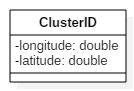
\includegraphics[width=0.2\linewidth]{images/database/classes/ClusterID}
\end{figure}
\subsubsection{Declaration}{
\begin{lstlisting}[frame=none]
public class ClusterID
 extends java.lang.Object\end{lstlisting}
\subsubsection{Constructor summary}{
\begin{verse}
\hyperlink{DatabaseConnection.ClusterID()}{{\bf ClusterID()}} Default constructor\\
\end{verse}
}
\subsubsection{Constructors}{
\vskip -2em
\begin{itemize}
\item{
\index{ClusterID()}
\hypertarget{DatabaseConnection.ClusterID()}{{\bf  ClusterID}\\}
\begin{lstlisting}[frame=none]
public ClusterID()\end{lstlisting} %end signature
\begin{itemize}
\item{
{\bf  Description}

Default constructor
}
\end{itemize}
}%end item
\end{itemize}
}
}
\newpage
\subsection{\label{DatabaseConnection.DataMaintainer}Class DataMaintainer}{
\hypertarget{DatabaseConnection.DataMaintainer}{}\vskip .1in
This class maintains the sensordata in the StorageSolution.\vskip .1in
\begin{figure}[!hbp]
	\centering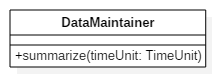
\includegraphics[width=0.3\linewidth]{images/database/classes/DataMaintainer}
\end{figure}
\subsubsection{Declaration}{
\begin{lstlisting}[frame=none]
public class DataMaintainer
 extends DatabaseConnection.Maintainer\end{lstlisting}
\subsubsection{Constructor summary}{
\begin{verse}
\hyperlink{DatabaseConnection.DataMaintainer()}{{\bf DataMaintainer()}} Default constructor\\
\end{verse}
}
\subsubsection{Method summary}{
\begin{verse}
\hyperlink{DatabaseConnection.DataMaintainer.summarize(TimeUnit)}{{\bf summarize(TimeUnit)}} This method takes data of a certain TimeUnit and summarizes it into the next higher TimeUnit.\\
\end{verse}
}
\subsubsection{Constructors}{
\vskip -2em
\begin{itemize}
\item{
\index{DataMaintainer()}
\hypertarget{DatabaseConnection.DataMaintainer()}{{\bf  DataMaintainer}\\}
\begin{lstlisting}[frame=none]
public DataMaintainer()\end{lstlisting} %end signature
\begin{itemize}
\item{
{\bf  Description}

Default constructor
}
\end{itemize}
}%end item
\end{itemize}
}
\subsubsection{Methods}{
\vskip -2em
\begin{itemize}
\item{
\index{summarize(TimeUnit)}
\hypertarget{DatabaseConnection.DataMaintainer.summarize(TimeUnit)}{{\bf  summarize}\\}
\begin{lstlisting}[frame=none]
public void summarize(TimeUnit timeUnit)\end{lstlisting} %end signature
\begin{itemize}
\item{
{\bf  Description}

This method takes data of a certain TimeUnit and summarizes it into the next higher TimeUnit. The summarized data is then saved back into the StorageSolution. The original data of the lower TimeUnit is then deleted from the database.
}
\item{
{\bf  Parameters}
  \begin{itemize}
   \item{
\texttt{timeUnit} -- The TimeUnit to summarize.}
  \end{itemize}
}%end item
\end{itemize}
}%end item
\end{itemize}
}
}
\subsection{\label{DatabaseConnection.Facade}Class Facade}{
\hypertarget{DatabaseConnection.Facade}{}\vskip .1in
A facade to simplify access to a StorageSolution, such as a database. Through the methods, data can be inserted into the StorageSolution and certain information about its content requested.\vskip .1in
\begin{figure}[!hbp]
	\centering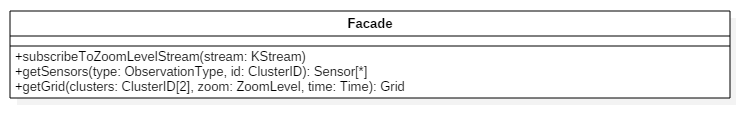
\includegraphics[width=0.9\linewidth]{images/database/classes/Facade}
\end{figure}
\subsubsection{Declaration}{
\begin{lstlisting}[frame=none]
public class Facade
 extends java.lang.Object\end{lstlisting}
\subsubsection{Constructor summary}{
\begin{verse}
\hyperlink{DatabaseConnection.Facade()}{{\bf Facade()}} Default constructor\\
\end{verse}
}
\subsubsection{Method summary}{
\begin{verse}
\hyperlink{DatabaseConnection.Facade.getGrid(DatabaseConnection.ClusterID[], DatabaseConnection.ZoomLevel, Time)}{{\bf getGrid(ClusterID\lbrack \rbrack , ZoomLevel, Time)}} Returns an appropriate grid of clusters in the requested grid section for the specified ZoomLevel and time.\\
\hyperlink{DatabaseConnection.Facade.getSensors(ObservationType, DatabaseConnection.ClusterID)}{{\bf getSensors(ObservationType, ClusterID)}} Fetches all sensors from the given cluster that observe the given ObservedProperty and returns an array of sensors.\\
\hyperlink{DatabaseConnection.Facade.subscribeToZoomLevelStream(KStream)}{{\bf subscribeToZoomLevelStream(KStream)}} Subscribes to the given KafkaStream, which contains ZoomLevel-specific data and initiates processing of its records.\\
\end{verse}
}
\subsubsection{Constructors}{
\vskip -2em
\begin{itemize}
\item{
\index{Facade()}
\hypertarget{DatabaseConnection.Facade()}{{\bf  Facade}\\}
\begin{lstlisting}[frame=none]
public Facade()\end{lstlisting} %end signature
\begin{itemize}
\item{
{\bf  Description}

Default constructor
}
\end{itemize}
}%end item
\end{itemize}
}
\subsubsection{Methods}{
\vskip -2em
\begin{itemize}
\item{
\index{getGrid(ClusterID\lbrack \rbrack , ZoomLevel, Time)}
\hypertarget{DatabaseConnection.Facade.getGrid(DatabaseConnection.ClusterID[], DatabaseConnection.ZoomLevel, Time)}{{\bf  getGrid}\\}
\begin{lstlisting}[frame=none]
public Grid getGrid(ClusterID[] clusters,ZoomLevel zoom,Time time)\end{lstlisting} %end signature
\begin{itemize}
\item{
{\bf  Description}

Returns an appropriate grid of clusters in the requested grid section for the specified ZoomLevel and time. The (first) two values of the ClusterID array define the grid section from which to get the data.
}
\item{
{\bf  Parameters}
  \begin{itemize}
   \item{
\texttt{clusters} -- An array of ClusterIDs from which the first two entries are taken to compute the section of the Grid to get the data from.}
   \item{
\texttt{zoom} -- The ZoomLevel from which to get the data.}
   \item{
\texttt{time} -- The point in time.}
  \end{itemize}
}%end item
\item{{\bf  Returns} --
A grid with the computed data.
}%end item
\end{itemize}
}%end item
\item{
\index{getSensors(ObservationType, ClusterID)}
\hypertarget{DatabaseConnection.Facade.getSensors(ObservationType, DatabaseConnection.ClusterID)}{{\bf  getSensors}\\}
\begin{lstlisting}[frame=none]
public java.util.Set getSensors(ObservationType type,ClusterID id)\end{lstlisting} %end signature
\begin{itemize}
\item{
{\bf  Description}

Fetches all sensors from the given cluster that observe the given ObservedProperty and returns an array of sensors.
}
\item{
{\bf  Parameters}
  \begin{itemize}
   \item{
\texttt{type} -- The ObservationType of the requested sensors.}
   \item{
\texttt{id} -- The ID of the cluster.}
  \end{itemize}
}%end item
\item{{\bf  Returns} --
An array of sensors.
}%end item
\end{itemize}
}%end item
\item{
\index{subscribeToZoomLevelStream(KStream)}
\hypertarget{DatabaseConnection.Facade.subscribeToZoomLevelStream(KStream)}{{\bf  subscribeToZoomLevelStream}\\}
\begin{lstlisting}[frame=none]
public void subscribeToZoomLevelStream(KStream stream)\end{lstlisting} %end signature
\begin{itemize}
\item{
{\bf  Description}

Subscribes to the given KafkaStream, which contains ZoomLevel-specific data and initiates processing of its records.
}
\item{
{\bf  Parameters}
  \begin{itemize}
   \item{
\texttt{stream} -- The stream to subscribe to.}
  \end{itemize}
}%end item
\end{itemize}
}%end item
\end{itemize}
}
}
\newpage
\subsection{\label{DatabaseConnection.GridDataServlet}Class GridDataServlet}{
\hypertarget{DatabaseConnection.GridDataServlet}{}\vskip .1in
An HTTPServlet for requesting Grid data.\vskip .1in
\begin{figure}[!hbp]
	\centering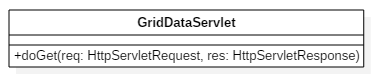
\includegraphics[width=0.6\linewidth]{images/database/classes/GridDataServlet}
\end{figure}
\subsubsection{Declaration}{
\begin{lstlisting}[frame=none]
public class GridDataServlet
 extends DatabaseConnection.HttpServlet\end{lstlisting}
\subsubsection{Constructor summary}{
\begin{verse}
\hyperlink{DatabaseConnection.GridDataServlet()}{{\bf GridDataServlet()}} Default constructor\\
\end{verse}
}
\subsubsection{Method summary}{
\begin{verse}
\hyperlink{DatabaseConnection.GridDataServlet.doGet(HttpServletRequest, HttpServletResponse)}{{\bf doGet(HttpServletRequest, HttpServletResponse)}} This method calls the getGrid method of the Facade to get a Grid of clusters at a certain ZoomLevel and Time .\\
\end{verse}
}
\subsubsection{Constructors}{
\vskip -2em
\begin{itemize}
\item{
\index{GridDataServlet()}
\hypertarget{DatabaseConnection.GridDataServlet()}{{\bf  GridDataServlet}\\}
\begin{lstlisting}[frame=none]
public GridDataServlet()\end{lstlisting} %end signature
\begin{itemize}
\item{
{\bf  Description}

Default constructor
}
\end{itemize}
}%end item
\end{itemize}
}
\subsubsection{Methods}{
\vskip -2em
\begin{itemize}
\item{
\index{doGet(HttpServletRequest, HttpServletResponse)}
\hypertarget{DatabaseConnection.GridDataServlet.doGet(HttpServletRequest, HttpServletResponse)}{{\bf  doGet}\\}
\begin{lstlisting}[frame=none]
public void doGet(HttpServletRequest req,HttpServletResponse res)\end{lstlisting} %end signature
\begin{itemize}
\item{
{\bf  Description}

This method calls the getGrid method of the Facade to get a Grid of clusters at a certain ZoomLevel and Time . This saves the Grid into res.
}
\item{
{\bf  Parameters}
  \begin{itemize}
   \item{
\texttt{req} -- An HttpServletRequest object that contains the request the client has made of the servlet.}
   \item{
\texttt{res} -- An HttpServletResponse object that contains the response the servlet sends to the client.}
  \end{itemize}
}%end item
\end{itemize}
}%end item
\end{itemize}
}
\subsubsection{Members inherited from class HttpServlet }{
\texttt{DatabaseConnection.HttpServlet} {\small
\refdefined{DatabaseConnection.HttpServlet}}
{\small

\vskip -2em
\begin{itemize}
\item{\vskip -1.5ex
\texttt{public void {\bf  doGet}(\texttt{HttpServletRequest} {\bf  req},
\texttt{HttpServletResponse} {\bf  res})
}%end signature
}%end item
\end{itemize}
}
}
\subsection{\label{DatabaseConnection.HttpServlet}Class HttpServlet}{
\hypertarget{DatabaseConnection.HttpServlet}{}\vskip .1in
An abstract HTTPServlet.\vskip .1in
\begin{figure}[!hbp]
	\centering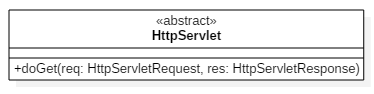
\includegraphics[width=0.6\linewidth]{images/database/classes/HttpServlet}
\end{figure}
\subsubsection{Declaration}{
\begin{lstlisting}[frame=none]
public class HttpServlet
 extends java.lang.Object\end{lstlisting}
\subsubsection{All known subclasses}{SensorListServlet\small{\refdefined{DatabaseConnection.SensorListServlet}}, GridDataServlet\small{\refdefined{DatabaseConnection.GridDataServlet}}}
\subsubsection{Constructor summary}{
\begin{verse}
\hyperlink{DatabaseConnection.HttpServlet()}{{\bf HttpServlet()}} Default constructor\\
\end{verse}
}
\subsubsection{Method summary}{
\begin{verse}
\hyperlink{DatabaseConnection.HttpServlet.doGet(HttpServletRequest, HttpServletResponse)}{{\bf doGet(HttpServletRequest, HttpServletResponse)}} Called by the server (via the service method) to allow a servlet to handle a GET request.\\
\end{verse}
}
\subsubsection{Constructors}{
\vskip -2em
\begin{itemize}
\item{
\index{HttpServlet()}
\hypertarget{DatabaseConnection.HttpServlet()}{{\bf  HttpServlet}\\}
\begin{lstlisting}[frame=none]
public HttpServlet()\end{lstlisting} %end signature
\begin{itemize}
\item{
{\bf  Description}

Default constructor
}
\end{itemize}
}%end item
\end{itemize}
}
\subsubsection{Methods}{
\vskip -2em
\begin{itemize}
\item{
\index{doGet(HttpServletRequest, HttpServletResponse)}
\hypertarget{DatabaseConnection.HttpServlet.doGet(HttpServletRequest, HttpServletResponse)}{{\bf  doGet}\\}
\begin{lstlisting}[frame=none]
public void doGet(HttpServletRequest req,HttpServletResponse res)\end{lstlisting} %end signature
\begin{itemize}
\item{
{\bf  Description}

Called by the server (via the service method) to allow a servlet to handle a GET request.
}
\item{
{\bf  Parameters}
  \begin{itemize}
   \item{
\texttt{req} -- An HttpServletRequest object that contains the request the client has made of the servlet.}
   \item{
\texttt{res} -- An HttpServletResponse object that contains the response the servlet sends to the client.}
  \end{itemize}
}%end item
\end{itemize}
}%end item
\end{itemize}
}
}
\subsection{\label{DatabaseConnection.KafkaToStorageProcessor}Class KafkaToStorageProcessor}{
\hypertarget{DatabaseConnection.KafkaToStorageProcessor}{}\vskip .1in
This class converts KafkaStream records to data that can be inserted into the StorageSolution.\vskip .1in
\begin{figure}[!hbp]
	\centering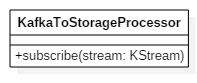
\includegraphics[width=0.3\linewidth]{images/database/classes/KafkaToStorageProcessor}
\end{figure}
\subsubsection{Declaration}{
\begin{lstlisting}[frame=none]
public class KafkaToStorageProcessor
 extends java.lang.Object\end{lstlisting}
\subsubsection{Constructor summary}{
\begin{verse}
\hyperlink{DatabaseConnection.KafkaToStorageProcessor()}{{\bf KafkaToStorageProcessor()}} Default constructor\\
\end{verse}
}
\subsubsection{Method summary}{
\begin{verse}
\hyperlink{DatabaseConnection.KafkaToStorageProcessor.subscribe(KStream)}{{\bf subscribe(KStream)}} Subscribes to the given KafkaStream and converts the data to the appropriate format for the StorageSolution.\\
\end{verse}
}
\subsubsection{Constructors}{
\vskip -2em
\begin{itemize}
\item{
\index{KafkaToStorageProcessor()}
\hypertarget{DatabaseConnection.KafkaToStorageProcessor()}{{\bf  KafkaToStorageProcessor}\\}
\begin{lstlisting}[frame=none]
public KafkaToStorageProcessor()\end{lstlisting} %end signature
\begin{itemize}
\item{
{\bf  Description}

Default constructor
}
\end{itemize}
}%end item
\end{itemize}
}
\subsubsection{Methods}{
\vskip -2em
\begin{itemize}
\item{
\index{subscribe(KStream)}
\hypertarget{DatabaseConnection.KafkaToStorageProcessor.subscribe(KStream)}{{\bf  subscribe}\\}
\begin{lstlisting}[frame=none]
public void subscribe(KStream stream)\end{lstlisting} %end signature
\begin{itemize}
\item{
{\bf  Description}

Subscribes to the given KafkaStream and converts the data to the appropriate format for the StorageSolution. If a stream is already subscribed to, unsubscribes from the old stream and subscribes to the new one.
}
\item{
{\bf  Parameters}
  \begin{itemize}
   \item{
\texttt{stream} -- The KStream to subscribe to.}
  \end{itemize}
}%end item
\end{itemize}
}%end item
\end{itemize}
}
}
\subsection{\label{DatabaseConnection.Maintainer}Class Maintainer}{
\hypertarget{DatabaseConnection.Maintainer}{}\vskip .1in
An abstract class describing a Maintainer, which performs maintenance on certain data in the StorageSolution.\vskip .1in
\begin{figure}[!hbp]
	\centering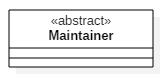
\includegraphics[width=0.25\linewidth]{images/database/classes/Maintainer}
\end{figure}
\subsubsection{Declaration}{
\begin{lstlisting}[frame=none]
public class Maintainer
 extends java.lang.Object\end{lstlisting}
\subsubsection{All known subclasses}{SensorMaintainer\small{\refdefined{DatabaseConnection.SensorMaintainer}}, DataMaintainer\small{\refdefined{DatabaseConnection.DataMaintainer}}}
\subsubsection{Constructor summary}{
\begin{verse}
\hyperlink{DatabaseConnection.Maintainer()}{{\bf Maintainer()}} Default constructor\\
\end{verse}
}
\subsubsection{Constructors}{
\vskip -2em
\begin{itemize}
\item{
\index{Maintainer()}
\hypertarget{DatabaseConnection.Maintainer()}{{\bf  Maintainer}\\}
\begin{lstlisting}[frame=none]
public Maintainer()\end{lstlisting} %end signature
\begin{itemize}
\item{
{\bf  Description}

Default constructor
}
\end{itemize}
}%end item
\end{itemize}
}
}
\subsection{\label{DatabaseConnection.MaintenanceManager}Class MaintenanceManager}{
\hypertarget{DatabaseConnection.MaintenanceManager}{}\vskip .1in
This class manages the way the methods of Maintainers are called to make sure the StorageSolution content is maintained.\vskip .1in
\begin{figure}[!hbp]
	\centering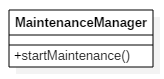
\includegraphics[width=0.25\linewidth]{images/database/classes/MaintenanceManager}
\end{figure}
\subsubsection{Declaration}{
\begin{lstlisting}[frame=none]
public class MaintenanceManager
 extends java.lang.Object\end{lstlisting}
\subsubsection{Constructor summary}{
\begin{verse}
\hyperlink{DatabaseConnection.MaintenanceManager()}{{\bf MaintenanceManager()}} Default constructor\\
\end{verse}
}
\subsubsection{Method summary}{
\begin{verse}
\hyperlink{DatabaseConnection.MaintenanceManager.startMaintenance()}{{\bf startMaintenance()}} This method should be called as soon as the database is started.\\
\end{verse}
}
\subsubsection{Constructors}{
\vskip -2em
\begin{itemize}
\item{
\index{MaintenanceManager()}
\hypertarget{DatabaseConnection.MaintenanceManager()}{{\bf  MaintenanceManager}\\}
\begin{lstlisting}[frame=none]
public MaintenanceManager()\end{lstlisting} %end signature
\begin{itemize}
\item{
{\bf  Description}

Default constructor
}
\end{itemize}
}%end item
\end{itemize}
}
\subsubsection{Methods}{
\vskip -2em
\begin{itemize}
\item{
\index{startMaintenance()}
\hypertarget{DatabaseConnection.MaintenanceManager.startMaintenance()}{{\bf  startMaintenance}\\}
\begin{lstlisting}[frame=none]
public void startMaintenance()\end{lstlisting} %end signature
\begin{itemize}
\item{
{\bf  Description}

This method should be called as soon as the database is started. Through calls to instances of Maintainers, summarizes data in the database and deletes data that has become obsolete as a result of the summarization.
}
\end{itemize}
}%end item
\end{itemize}
}
}
\subsection{\label{DatabaseConnection.SensorListServlet}Class SensorListServlet}{
\hypertarget{DatabaseConnection.SensorListServlet}{}\vskip .1in
An HTTPServlet for requesting a list of sensors.\vskip .1in
\begin{figure}[!hbp]
	\centering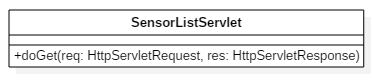
\includegraphics[width=0.6\linewidth]{images/database/classes/SensorListServlet}
\end{figure}
\subsubsection{Declaration}{
\begin{lstlisting}[frame=none]
public class SensorListServlet
 extends DatabaseConnection.HttpServlet\end{lstlisting}
\subsubsection{Constructor summary}{
\begin{verse}
\hyperlink{DatabaseConnection.SensorListServlet()}{{\bf SensorListServlet()}} Default constructor\\
\end{verse}
}
\subsubsection{Method summary}{
\begin{verse}
\hyperlink{DatabaseConnection.SensorListServlet.doGet(HttpServletRequest, HttpServletResponse)}{{\bf doGet(HttpServletRequest, HttpServletResponse)}} This method calls the getSensors method of the Facade to get a list of Sensors that are in a certain cluster.\\
\end{verse}
}
\subsubsection{Constructors}{
\vskip -2em
\begin{itemize}
\item{
\index{SensorListServlet()}
\hypertarget{DatabaseConnection.SensorListServlet()}{{\bf  SensorListServlet}\\}
\begin{lstlisting}[frame=none]
public SensorListServlet()\end{lstlisting} %end signature
\begin{itemize}
\item{
{\bf  Description}

Default constructor
}
\end{itemize}
}%end item
\end{itemize}
}
\subsubsection{Methods}{
\vskip -2em
\begin{itemize}
\item{
\index{doGet(HttpServletRequest, HttpServletResponse)}
\hypertarget{DatabaseConnection.SensorListServlet.doGet(HttpServletRequest, HttpServletResponse)}{{\bf  doGet}\\}
\begin{lstlisting}[frame=none]
public void doGet(HttpServletRequest req,HttpServletResponse res)\end{lstlisting} %end signature
\begin{itemize}
\item{
{\bf  Description}

This method calls the getSensors method of the Facade to get a list of Sensors that are in a certain cluster.
}
\item{
{\bf  Parameters}
  \begin{itemize}
   \item{
\texttt{req} -- An HttpServletRequest object that contains the request the client has made of the servlet.}
   \item{
\texttt{res} -- An HttpServletResponse object that contains the response the servlet sends to the client.}
  \end{itemize}
}%end item
\end{itemize}
}%end item
\end{itemize}
}
\subsubsection{Members inherited from class HttpServlet }{
\texttt{DatabaseConnection.HttpServlet} {\small
\refdefined{DatabaseConnection.HttpServlet}}
{\small

\vskip -2em
\begin{itemize}
\item{\vskip -1.5ex
\texttt{public void {\bf  doGet}(\texttt{HttpServletRequest} {\bf  req},
\texttt{HttpServletResponse} {\bf  res})
}%end signature
}%end item
\end{itemize}
}
}
\subsection{\label{DatabaseConnection.SensorMaintainer}Class SensorMaintainer}{
\hypertarget{DatabaseConnection.SensorMaintainer}{}\vskip .1in
This class maintains the list of sensors saved in the StorageSolution.\vskip .1in
\begin{figure}[!hbp]
	\centering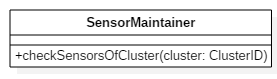
\includegraphics[width=0.4\linewidth]{images/database/classes/SensorMaintainer}
\end{figure}
\subsubsection{Declaration}{
\begin{lstlisting}[frame=none]
public class SensorMaintainer
 extends DatabaseConnection.Maintainer\end{lstlisting}
\subsubsection{Constructor summary}{
\begin{verse}
\hyperlink{DatabaseConnection.SensorMaintainer()}{{\bf SensorMaintainer()}} Default constructor\\
\end{verse}
}
\subsubsection{Method summary}{
\begin{verse}
\hyperlink{DatabaseConnection.SensorMaintainer.checkSensorsOfCluster(DatabaseConnection.ClusterID)}{{\bf checkSensorsOfCluster(ClusterID)}} This method checks if the sensors registered to the given cluster are up to date.\\
\end{verse}
}
\subsubsection{Constructors}{
\vskip -2em
\begin{itemize}
\item{
\index{SensorMaintainer()}
\hypertarget{DatabaseConnection.SensorMaintainer()}{{\bf  SensorMaintainer}\\}
\begin{lstlisting}[frame=none]
public SensorMaintainer()\end{lstlisting} %end signature
\begin{itemize}
\item{
{\bf  Description}

Default constructor
}
\end{itemize}
}%end item
\end{itemize}
}
\subsubsection{Methods}{
\vskip -2em
\begin{itemize}
\item{
\index{checkSensorsOfCluster(ClusterID)}
\hypertarget{DatabaseConnection.SensorMaintainer.checkSensorsOfCluster(DatabaseConnection.ClusterID)}{{\bf  checkSensorsOfCluster}\\}
\begin{lstlisting}[frame=none]
public void checkSensorsOfCluster(ClusterID cluster)\end{lstlisting} %end signature
\begin{itemize}
\item{
{\bf  Description}

This method checks if the sensors registered to the given cluster are up to date. A sensor is up to date if data has been received from it in the last 24 hours. If this requirement is not met, the sensor is deleted from the database.
}
\item{
{\bf  Parameters}
  \begin{itemize}
   \item{
\texttt{cluster} -- The cluster to check.}
  \end{itemize}
}%end item
\end{itemize}
}%end item
\end{itemize}
}
}
\subsection{\label{DatabaseConnection.ZoomLevel}Class ZoomLevel}{
\hypertarget{DatabaseConnection.ZoomLevel}{}\vskip .1in
This class describes a zoom level for the map.\vskip .1in
\begin{figure}[!hbp]
	\centering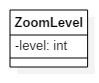
\includegraphics[width=0.15\linewidth]{images/database/classes/ZoomLevel}
\end{figure}
\subsubsection{Declaration}{
\begin{lstlisting}[frame=none]
public class ZoomLevel
 extends java.lang.Object\end{lstlisting}
\subsubsection{Constructor summary}{
\begin{verse}
\hyperlink{DatabaseConnection.ZoomLevel()}{{\bf ZoomLevel()}} Default constructor\\
\end{verse}
}
\subsubsection{Constructors}{
\vskip -2em
\begin{itemize}
\item{
\index{ZoomLevel()}
\hypertarget{DatabaseConnection.ZoomLevel()}{{\bf  ZoomLevel}\\}
\begin{lstlisting}[frame=none]
public ZoomLevel()\end{lstlisting} %end signature
\begin{itemize}
\item{
{\bf  Description}

Default constructor
}
\end{itemize}
}%end item
\end{itemize}
}
}
}
